\documentclass{article}
\usepackage[utf8]{inputenc}
\usepackage{amsmath}
\usepackage{longtable}
\usepackage{import}
\usepackage{hyperref}
\usepackage[compact]{titlesec}
\usepackage{booktabs}
\usepackage{graphicx}
\usepackage{amssymb}

\title{SOEN 6481 - Software Requirement Specification}
\author{Project Deliverable 2 by Sarvesh Vora}
\date{August 2, 2019}
\newcommand\tab[1][1cm]{\hspace*{#1}}

\begin{document}
\maketitle
\pagenumbering{arabic}
\newpage
\tableofcontents
\newpage
\section{Problem 6:}
\subsection{Important Tables:}
\subsubsection{Interview Details:}
\begin{table}[h!]
    \begin{tabular}{|| l|| l ||}
        \hline
         Interview ID & Details  \\
         \hline
         I1 & Prof. Bhupendra Kesaria \\
         \hline
         I2 & Alexandros Mavrias \\
         \hline
    \end{tabular}
\end{table}
\subsubsection{Survey Details:}
\begin{table}[h!]
    \begin{tabular}{|| l || l || }
        \hline
        Survey ID & Details \\
        \hline
        S1 & Sushila Vora \\ 
        \hline
        S2 & Shivam Patel \\ 
        \hline
        S3 & Prof. Bhupendra Kesaria \\ 
        \hline
        S4 & Alexandros Mavrias \\ 
        \hline
    \end{tabular}
\end{table}
\subsubsection{Calculator Details:}
\begin{table}[h!]
    \begin{tabular}{|| l || l || }
        \hline
        Calculator ID & Details \\
        \hline
        C1 & Scientific Calculator \\ 
        \hline
        C2 & Business Calculator \\ 
        \hline
    \end{tabular}
\end{table}
\subsubsection{Error Details:}
\begin{table}[h!]
    \begin{tabular}{|| l || l || }
        \hline
        Error Code & Error Message \\
        \hline
        E1 & Invalid operand. \\ 
        \hline
        E2 & Multiple Operator. \\ 
        \hline
        E3 & Interest rate out of range. \\ 
        \hline
        E4 & Time out \\ 
        \hline
    \end{tabular}
\end{table}
\newpage
\subsubsection{Online Link Details:}
\begin{table}[h!]
    \begin{tabular}{|| l || l || }
        \hline
        Link ID & Details \\
        \hline
        L1 & \href{http://www.slideshare.net/DhavalDalal/calculator-stories}{Slide Share - Dhaval Dalal} \\ 
        \hline
        L2 &  \href{http://www2.southeastern.edu/Academics/Faculty/dgurney/Math241/StatTopics/SciNot.htm}{South Eastern} \\
        \hline
        L3 & \href{http://www.miniwebtool.com/}{Mini Web Tool} \\ 
        \hline
        L4 & \href{https://en.wikipedia.org/wiki/Natural_logarithm_of_2}{Wiki - Natural log of 2} \\ 
        \hline
        L5 & \href{http://mathworld.wolfram.com/NaturalLogarithmof2.html}{Math World - Natural log of 2} \\ 
        \hline
        L6 & \href{https://www.patriotsoftware.com/accounting/training/blog/how-do-you-determine-a-profit-margin/}{Patriot Software - Calculate Profit} \\ 
        \hline
        L7 & \href{https://en.wikipedia.org/wiki/E_(mathematical_constant)}{Wiki - Math Constant $e$} \\ 
        \hline
        L8 & \href{https://www.investopedia.com/terms/r/ruleof72.asp}{Investopedia - Rule of 72} \\ 
        \hline
    \end{tabular}
\end{table}
\subsection{Field Information:}
\subsubsection{Priority: }
\tab[1.2cm] The priority is based on how a user story is essential for the system. High describes highest priority and low to specify least priority.
For an example, Addition and Subtraction are core operations of a calculator without which calculator can not work but Multiplication or Division can be achieved by successively do addition or subtraction. Therefore Addition and Subtraction has high priority whereas Multiplication and Division has Medium priority.
\subsubsection{Estimate: }
\tab[1.2cm] An Estimate is one of the number from Fibonacci sequence. Where the number 1 in Fibonacci sequence represents 10 minutes of time. An Estimate is derived depending on the complexity of the user story implementation, its acceptance test(s) and development environment. 
\\ \\ \\
\noindent
\textbf{NOTE : } Please check Appendix A and Appendix B for additional Interview and Survey respectively. The interview got delayed due to unavailability of the interviewee before the deliverable 1 deadline. Furthermore, to gain some extra knowledge to build atomic user stories, I have conducted a survey. 
\newpage
\subsection{User Story : }
\begin{longtable}{|| c || l ||}
        \hline
        \hline
        \textbf{User Story ID} & \textbf{Description} \\
        \hline
        \hline
         US1 & \textbf{Theme} : Operand \\
         & \textbf{Constraint} : As a user I should be able to enter 0 to 9 digits or \\ & '.' decimal point as an operand only. \\ 
         & \textbf{Priority} : High \\
         & \textbf{Estimate} : 5 \\
         & \textbf{Acceptance Test} : Given, If any character is entered as an \\
         & operand except for digits or '.' then show Error: E1 \\
         & \textbf{Constraints: } While input a user shall only enter real numbers.\\
         & \textbf{Sources} : \\
         & 1.~Sarvesh Vora - intuition \\
         \hline
         US2 & \textbf{Theme} : Operator \\
         & \textbf{Constraint} : As a user I want addition operator to add two \\
         & integers. \\
         & \textbf{Priority} : High \\
         & \textbf{Estimate} : 1 \\
         & \textbf{Acceptance Test} : Accept two integers, let's say 2 and 3 then it \\
         & should produce 5 as an output. \\
         & \textbf{Constraints: } Both the numbers shall be real numbers.\\
         & \textbf{Sources} : \\
         & 1.~L1 \\
         \hline
         US3 & \textbf{Theme} : Operator \\
         & \textbf{Constraint} : As a user I want subtraction operator to minus one \\ 
         & Integer from another. \\
         & \textbf{Priority} : High \\
         & \textbf{Estimate} : 1 \\
         & \textbf{Acceptance Test} : Accept two integers, let's say 2 and 3 then it \\
         & should produce -1 as an output. \\
         & \textbf{Constraints: } Both the numbers shall be real numbers.\\
         & \textbf{Sources} : \\
         & 1.~L1 \\
         \hline
         US4 & \textbf{Theme} : Operator \\
         & \textbf{Constraint} : As a user I need a '.' Operator for decimal input. \\ 
         & \textbf{Priority} : High \\
         & \textbf{Estimate} : 2 \\
         & \textbf{Acceptance Test} : Given, if user presses '.' key then It shall \\ 
         & print one '.' and if more than one then show Error: E1. \\
         & \textbf{Constraints: } There will always be only one decimal point.\\
         & \textbf{Sources} : \\
         & 1.~L2 \\
         \hline
         \newpage
         \hline
         US5 & \textbf{Theme} : Display \\
         & \textbf{Constraint} : As a user when I give any input, it should reflect \\ 
         & on the display.\\ 
         & \textbf{Priority} : High \\
         & \textbf{Estimate} : 0 \\
         & \textbf{Acceptance Test} : Given, if user presses any key it shall be \\ 
         & displayed on the screen.\\
         & \textbf{Sources} : \\
         & 1.~Sarvesh Vora - intuition \\
         \hline
         US6 & \textbf{Theme} : Validation \\
         & \textbf{Constraint} : As a Programmer, my program should not accept a \\
         & number to begin with multiple zeros. \\
         & \textbf{Priority} : High \\
         & \textbf{Estimate} : 8 \\
         & \textbf{Acceptance Test} : Accept an integer, if it begins with zeros \\
         & then Show Error: E1.\\
         & \textbf{Sources} : \\
         & 1.~Sarvesh Vora - intuition \\
         \hline
         US7 & \textbf{Theme} : Validation \\
         & \textbf{Constraint} : As a programmer, My program should not accept \\ 
         & operand other than digits and ANS. \\
         & \textbf{Priority} : High \\
         & \textbf{Estimate} : 3 \\
         & \textbf{Acceptance Test} : Given, A user is only allowed to put one \\
         & operator per operation, if more Show Error: E2.\\
         & \textbf{Constraints: } The number shall be real number or ANS.\\
         & \textbf{Sources} : \\
         & 1.~Sarvesh Vora - intuition \\
         \hline
         US8 & \textbf{Theme} : Validation \\
         & \textbf{Constraint} : As a programmer, If the denominator is zero in \\ 
         & division then answer should be zero.\\
         & \textbf{Priority} : High \\
         & \textbf{Estimate} : 3 \\
         & \textbf{Acceptance Test} : If the denominator is zero then program \\ 
         & should display Infinity on screen as an output.\\
         & \textbf{Constraints: } Denominator can not be zero.\\
         & \textbf{Sources} : \\
         & 1.~L1 \\
         & 2.~US25 \\
         \hline
         \newpage
         \hline
         US9 & \textbf{Theme} : Decimal \\
         & \textbf{Constraint} : As a Student, I want upto 6 digits after the \\ 
         & decimal point. \\ 
         & \textbf{Priority} : High \\
         & \textbf{Estimate} : 5 \\
         & \textbf{Acceptance Test} : The program shall display upto 6 digits \\ 
         & and trim rest all. \\
         & \textbf{Sources} : \\
         & 1.~S2 \\
         \hline
         US10 & \textbf{Theme} : Decimal \\
         & \textbf{Constraint} : As a Teacher, I want upto 6 digits after the decimal \\
         & point. \\ 
         & \textbf{Priority} : High \\
         & \textbf{Estimate} : 5 \\
         & \textbf{Acceptance Test} : The program shall display upto 6 digits \\ 
         & and trim rest all. \\
         & \textbf{Sources} : \\
         & 1.~S3 \\
         \hline
         US11 & \textbf{Theme} : Decimal \\
         & \textbf{Constraint} : As a Housewife, I want upto 2 digits after the\\ 
         & decimal point. \\ 
         & \textbf{Priority} : High \\
         & \textbf{Estimate} : 5 \\
         & \textbf{Acceptance Test} : The program shall display upto 2 digits \\ 
         & and trim rest all. \\
         & \textbf{Sources} : \\
         & 1.~S1 \\
         \hline
         US12 & \textbf{Theme} : Decimal \\
         & \textbf{Constraint} : As an Investment Analyst, I'd like upto 4 \\ 
         & digits after the decimal point. \\
         & \textbf{Priority} : High \\
         & \textbf{Estimate} : 5 \\
         & \textbf{Acceptance Test} : The program shall display upto 4 digits \\ 
         & and trim rest all. \\
         & \textbf{Sources} : \\
         & 1.~S4 \\
         \hline
         \newpage
         \hline
         US13 & \textbf{Theme} : Validation \\
         & \textbf{Constraint} : As a programmer, I'd expect that the rate of \\ 
         & interest will be between 1\% to 100\%.\\ 
         & \textbf{Priority} : High \\
         & \textbf{Estimate} : 8 \\
         & \textbf{Acceptance Test} : Given the rate of interest, if not within \\ 
         & the range of 1\% to 100\% then Show Error: E3. \\
         & \textbf{Constraints: } Any real number between 1 to 100.\\
         & \textbf{Sources} : \\
         & 1.~I2 \\
         \hline
         US14 & \textbf{Theme} : Finance \\
         & \textbf{Constraint} : As an Investment Analyst, I'd like to get the \\ 
         & result within 0.1 second because of market price fluctuation.\\ 
         & \textbf{Priority} : High \\
         & \textbf{Estimate} : 8 \\
         & \textbf{Acceptance Test} : Given any operation, the result shall be \\ 
         & displayed within 0.1 seconds else show Error: E4 . \\
         & \textbf{Constraints: } Response time shall be less than 0.1 second.\\
         & \textbf{Sources} : \\
         & 1.~I2 \\
         \hline
         US15 & \textbf{Theme} : Power \\
         & \textbf{Constraint} : As a user, I need power on/off switch to \\ 
         & start and stop calculator.\\
         & \textbf{Priority} : High \\
         & \textbf{Estimate} : 8 \\
         & \textbf{Acceptance Test} : When pressed on or off the calculator \\
         & shall start or stop execution respectively.\\
         & \textbf{Sources} : \\
         & 1.~I2 \\
         \hline
         US16 & \textbf{Theme} : Operator \\
         & \textbf{Constraint} : As a user I want modulus operator to get \\
         & the remainder after division.\\
         & \textbf{Priority} : Low \\
         & \textbf{Estimate} : 1 \\
         & \textbf{Acceptance Test} : Accept two Integer, lets say 10 and 3, it shall\\
         & produce 1 as an output.\\
         & \textbf{Constraints: } Both the numbers shall be real numbers\\
         & and denominator can not be equal to zero..\\
         & \textbf{Sources} : \\
         & 1.~L3 \\
         & 2~US25 \\
         \hline
         \newpage
         \hline
         US17 & \textbf{Theme} : Operator \\
         & \textbf{Constraint} : As a user I'd like an ANS operator to preserve my \\
         & previous answer.\\
         & \textbf{Priority} : Low \\
         & \textbf{Estimate} : 3 \\
         & \textbf{Acceptance Test} : After every operation, the answer shall be \\
         & stored in ANS and displayed whenever used.\\
         & \textbf{Sources} : \\
         & 1.~Sarvesh Vora - intuition \\
         \hline
         US18 & \textbf{Theme} : Operator \\
         & \textbf{Constraint} : As a student, I'd like to have '!' operator for \\
         & factorial.\\
         & \textbf{Priority} : Low \\
         & \textbf{Estimate} : 2 \\
         & \textbf{Acceptance Test} : Given an Integer, display the factorial \\
         & value of the integer.\\
         & \textbf{Constraints: } The number shall be real number.\\
         & \textbf{Sources} : \\
         & 1.~L3 \\
         \hline
         US19 & \textbf{Theme} : Operator \\
         & \textbf{Constraint} : As a student, I need logarithm operator to \\
         & calculate growth.\\
         & \textbf{Priority} : Low \\
         & \textbf{Estimate} : 3 \\
         & \textbf{Acceptance Test} : Given an Integer n, Display the value of\\
         & log(n) to the base 10.\\
         & \textbf{Constraints: } The number shall be real number.\\
         & \textbf{Sources} : \\
         & 1.~C1 \\
         \hline
         US20 & \textbf{Theme} : Operator \\
         & \textbf{Constraint} : As a student, I need value of 'e'.\\
         & \textbf{Priority} : Low \\
         & \textbf{Estimate} : 1 \\
         & \textbf{Acceptance Test} : Display the value of e =  2.71828\\
         & \textbf{Constraints: } The value of e shall be accurate till \\
         & 6 digits after decimal.\\
         & \textbf{Sources} : \\
         & 1.~L7 \\
        \hline
        \newpage
        \hline
         US21 & \textbf{Theme} : Operator \\
         & \textbf{Constraint} : As a student, I'd like to have '$\wedge$' operator\\
         & to perform raise to operation.\\
         & \textbf{Priority} : Low \\
         & \textbf{Estimate} : 2 \\
         & \textbf{Acceptance Test} : Given two Integer x \& y, display value\\
         & of x raise to y.\\
         & \textbf{Constraints: } Both the numbers shall be real numbers.\\
         & \textbf{Sources} : \\
         & 1.~L3 \\
         \hline
         US22 & \textbf{Theme} : Operator \\
         & \textbf{Constraint} : As an Investment Analyst, I need 'Round' \\
         & operator to round off the decimal points.\\
         & \textbf{Priority} : Low \\
         & \textbf{Estimate} : 5 \\
         & \textbf{Acceptance Test} : Given a fractional number, round it \\
         & off depending on the decimal value.\\
         & \textbf{Sources} : \\
         & 1.~C2 \\
         & 2.~I2 \\
         \hline
         US23 & \textbf{Theme} : History \\
         & \textbf{Constraint} : As a user, I'd like to see history of \\
         & the operations I did.\\
         & \textbf{Priority} : Low \\
         & \textbf{Estimate} : 8 \\
         & \textbf{Acceptance Test} : After every operation, the operation \\
         & shall be stored and displayed when required.\\
         & \textbf{Sources} : \\
         & 1.~Sarvesh Vora - intuition \\
         \hline
         US24 & \textbf{Theme} : Operator \\
         & \textbf{Constraint} : As a user I want multiplication operator \\
         & to multiply an Integer by another.\\
         & \textbf{Priority} : Medium \\
         & \textbf{Estimate} : 1 \\
         & \textbf{Acceptance Test} : Given two integer lets say 3 and 4, \\
         & it shall produce 12 as an output.\\
         & \textbf{Constraints: } Both the numbers shall be real numbers.\\
         & \textbf{Sources} : \\
         & 1.~L1 \\
         \hline
         \newpage
         \hline
         US25 & \textbf{Theme} : Operator \\
         & \textbf{Constraint} : As a user I want division operator to \\
         & divide an integer by another.\\
         & \textbf{Priority} : Medium \\
         & \textbf{Estimate} : 1 \\
         & \textbf{Acceptance Test} : Given two integer lets say 12 and 4,\\
         & it shall produce 3 as an output.\\
         & \textbf{Constraints: } Both the numbers shall be real numbers and \\
         & denominator shall not be zero.\\
         & \textbf{Sources} : \\
         & 1.~L1 \\
         \hline
         US26 & \textbf{Theme} : Operator \\
         & \textbf{Constraint} : As a student, I want a "clear" operator,\\
         & to clear screen.\\
         & \textbf{Priority} : Medium \\
         & \textbf{Estimate} : 5 \\
         & \textbf{Acceptance Test} : When pressed, it shall clear history\\
         & and clear the screen.\\
         & \textbf{Sources} : \\
         & 1.~Sarvesh Vora - intuition \\
         \hline
         \hline
         US27 & \textbf{Theme} : Finance \\
         & \textbf{Constraint} : As an Investment Analyst, I'd like to have \\
         & value of natural log of 2 to calculate 'Rule of 72'.\\
         & \textbf{Priority} : Medium \\
         & \textbf{Estimate} : 3 \\
         & \textbf{Acceptance Test} : Derive the value of $\ln(n)$ = 0.693147\\
         & \textbf{Constraints: } The value of natural log of 2 shall be \\
         & accurate till 4 digits after decimal.\\
         & \textbf{Sources} : \\
         & 1.~L4\\
         & 2.~L5\\
         \hline
         US28 & \textbf{Theme} : Operation \\
         & \textbf{Constraint} : As an Investment Analyst, I need 'Rule of 72' \\
         & function to calculate time to double money.\\
         & \textbf{Priority} : Medium \\
         & \textbf{Estimate} : 8 \\
         & \textbf{Acceptance Test} : Given rate of interest, display the time\\
         & require to double money at interest rate.\\
         & \textbf{Sources} : \\
         & 1.~L8\\
         & 2.~US27\\
         & 3.~I2 \\
         \hline
         \newpage
         \hline
         US29 & \textbf{Theme} : Operation \\
         & \textbf{Constraint} : As an Investment Analyst, I want to calculate \\
         & profit using 'profit' option.\\
         & \textbf{Priority} : Medium \\
         & \textbf{Estimate} : 8 \\
         & \textbf{Acceptance Test} : Given net income and revenue, calculate\\
         & profit margin.\\
         & \textbf{Constraints: } Both the values shall be real numbers.\\
         & \textbf{Sources} : \\
         & 1.~L6\\
         & 2.~I2 \\
         \hline
         US30 & \textbf{Theme} : Operation \\
         & \textbf{Constraint} : As a student, I need parentheses '(' \& ')' \\
         & for forming expression.\\
         & \textbf{Priority} : Medium \\
         & \textbf{Estimate} : 13 \\
         & \textbf{Acceptance Test} : Given an expression with parentheses, \\
         & the parentheses shall evaluated first.\\
         & \textbf{Sources} : \\
         & 1.~Sarvesh Vora - intuition\\
         \hline
         US31 & \textbf{Theme} : Operation \\
         & \textbf{Constraint} : As a user, I need $\log_{10}(n)$ function to calculate\\
         & the value of $\log_{10}(n)$.\\
         & \textbf{Priority} : Medium \\
         & \textbf{Estimate} : 3 \\
         & \textbf{Acceptance Test} : Given value of n, where n is a real number,\\
         & it shall give correct value.\\
         & \textbf{Constraints: } It shall be accurate till 6 digits after the decimal.\\
         & \textbf{Sources} : \\
         & 1.~C1\\
         \hline
         US32 & \textbf{Theme} : Operation \\
         & \textbf{Constraint} : As a user, I need a $\ln(n)$ function to \\
         & calculate Natural logarithm of n.\\
         & \textbf{Priority} : Medium \\
         & \textbf{Estimate} : 3 \\
         & \textbf{Acceptance Test} : Given the value of n, where n is a real number, \\
         & it shall provide correct value of $\ln{n}$.\\
         & \textbf{Constraints: } It shall be accurate till 6 digits after the decimal.\\
         & \textbf{Sources} : \\
         & 1.~C1\\
         & 2.~US31 \\
         \hline
         \hline
\end{longtable}
\newpage
\section{Problem 7:}
\subsection{Traceability Matrix}
\begin{longtable}{ || l | l | l | l | l | l | l | l ||}
        \hline
        US ID & Sarvesh Vora - intuition & User Story & Survey & Interview & Links & Calculator \\ 
        \hline
        US1 & \checkmark &  &  &  &  &  \\ 
        \hline
        US2 &  &  &  &  & \checkmark -L1 &  \\ 
        \hline
        US3 &  &  &  &  & \checkmark -L1 &  \\ 
        \hline
        US4 &  &  &  &  & \checkmark -L2 &  \\ 
        \hline
        US5 & \checkmark &  &  &  &  &  \\ 
        \hline
        US6 & \checkmark &  &  &  &  &  \\ 
        \hline
        US7 & \checkmark &  &  &  &  &  \\ 
        \hline
        US8 &  & \checkmark -US25 &  &  & \checkmark -L1 &  \\ 
        \hline
        US9 &  &  & \checkmark -S2 &  &  &  \\ 
        \hline
        US10 &  &  & \checkmark -S3 &  &  &  \\ 
        \hline
        US11 &  &  & \checkmark -S1 &  &  &  \\ 
        \hline
        US12 &  &  & \checkmark -S4 &  &  &  \\ 
        \hline
        US13 &  &  &  & \checkmark -I2 &  &  \\ 
        \hline
        US14 &  &  &  & \checkmark -I2 &  &  \\ 
        \hline
        US15 & \checkmark &  &  &  &  &  \\ 
        \hline
        US16 &  & \checkmark -US25 &  &  & \checkmark -L3 &  \\ 
        \hline
        US17 & \checkmark &  &  &  &  &  \\ 
        \hline
        US18 &  &  &  &  & \checkmark -L3 &  \\ 
        \hline
        US19 &  &  &  &  &  & \checkmark -C1 \\ 
        \hline
        US20 &  &  &  &  & \checkmark -L7 &  \\ 
        \hline
        US21 &  &  &  &  & \checkmark -L3 &  \\ 
        \hline
        US22 &  &  &  &  &  & \checkmark -C2 \\ 
        \hline
        US23 & \checkmark &  &  &  &  &  \\ 
        \hline
        US24 &  &  &  &  & \checkmark -L1 &  \\ 
        \hline
        US25 &  &  &  &  & \checkmark -L1 &  \\ 
        \hline
        US26 & \checkmark &  &  & \checkmark -I1 &  &  \\ 
        \hline
        US27 &  & \checkmark -US32 &  &  & \checkmark -L4 -L5 &  \\ 
        \hline
        US28 &  & \checkmark -US27 &  & \checkmark -I2 & \checkmark -L8 &  \\ 
        \hline
        US29 &  &  &  & \checkmark -I2 & \checkmark -L6 &  \\ 
        \hline
        US30 & \checkmark &  &  &  &  &  \\ 
        \hline
        US31 &  &  &  &  &  & \checkmark -C1 \\ 
        \hline
        US32 &  & \checkmark -US31 &  &  &  & \checkmark -C1 \\ 
        \hline
\end{longtable}

\newpage
\section{Problem 8:}
\subsection{Important Information:}
\textbf{JAR file:} CalcUS.jar \\ \\
\textbf{Command:} java -jar CalcUS.jar \\ \\
\textbf{Java Document:} Kindly go to JavaDoc folder and double click on index.html and check on your browser. \\


\newpage
\subsection{Class Diagram:}
\begin{figure}[h!]
    \centering
    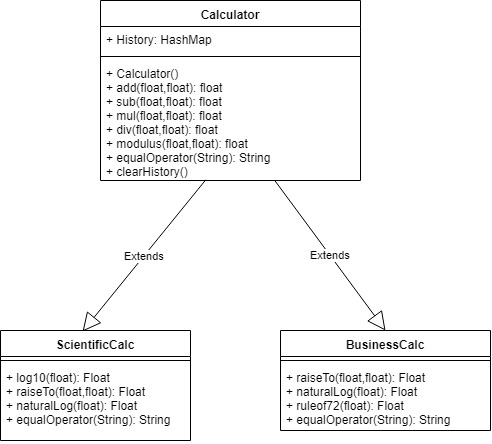
\includegraphics[scale=0.90]{Problem_8.jpg}
\end{figure}


\newpage
\section{Appendix A: Interview}
\subsection{Interviewee Information:}
\textbf{Name:} Alexandros Mavrias \\
\textbf{Email:} a\_mavrias@hotmail.com \\
\textbf{Gender:} Male \\
\textbf{Age:} 37 \\
\textbf{Profession:} Investment Analyst \\
\textbf{Bio :} Alexandros has done B.Com. and MBA from McGill university. He has created financial models to determine the feasibility of joint ventures with international partners and capital investment projects for the company’s network of global training centers. He performed fundamental analysis of US and Latin American companies operating in the financial, energy, material and utility sectors. He has developed financial models to determine the intrinsic value of companies, including sensitivity and scenario analysis.

\subsection{Interview QnA:}
\noindent
\textbf{Q1: } What's your good name? \\
\textbf{A1 : } Alexandros Mavrias. \\ \\
\textbf{Q2: } What line of work are you in? \\
\textbf{A2 : } I am an Investment Analyst.\\ \\
\textbf{Q3: } Where do you work? \\
\textbf{A3 : } National Bank Financial.\\ \\
\textbf{Q4: } Do you use a Financial calculator? \\
\textbf{A4 : } Yes, indeed its really helpful.\\ \\
\textbf{Q5: } How quick you want your calculator to be? \\
\textbf{A5 : } I want my calculator to be really quick like a split of seconds because I deal with stock market and investment market and I require quick response from the calculator to take the decisions as quick as possible.\\ \\
\textbf{Q6: } What are most often used operations that you perform over the financial calculator? \\
\textbf{A6 : } Things which are related to investment, like calculating the time require to increase the principal amount, Approximation, round off, calculating profit, calculating depreciation, etc. \\ \\
\textbf{Q7: } Oh, You use round off more often, Why? \\
\textbf{A7 : } Usually we cant always tell the exact time or maturity date for the client's investment so we round it off to the floor value of any fraction. to achieve a base idea of time. \\ \\
\textbf{Q8: } How do you calculate profit? \\
\textbf{A8 : } I actually calculate the profit margin and then apply it to the principal amount. Its easy to calculate the profit margin. All you to do is calculate the net income and revenue. Divide the net income by revenue. finally multiply the answer by 100. \\ \\
\textbf{Q9: } Do you use natural logarithm of 2 $\ln(n)$ in your calculations? \\
\textbf{A9 : } Yes, We use it in calculating the Rule of 72. \\ \\
\textbf{Q10: } What is rule of 72? \\
\textbf{A10 : } The Rule of 72 is a quick, useful formula that is used to estimate the number of years required to double the invested money at a given annual rate of return. \\ \\
\textbf{Q11: } What is rate of interest and whats it's range? \\
\textbf{A11 : } A rate of interest (RoI) is the net gain or loss on an investment over a specified time period, expressed as a percentage of the investment’s initial cost. It can be from 1\% to 100\%. \\ \\
\textbf{Q11: } How do we calculate rule of 72? \\
\textbf{A11 : } You need the value of r that you need to put it into a formula, which is, \\
$T \simeq \frac{\ln(2)}{\ln(1+\frac{r}{100})}$
    where: \\
    T = Time to double the money. \\
    r = Compounded interest rate per period. \\ \\



\newpage
\section{Appendix B: Survey}
\subsection{Survey Questions :}
\textbf{Question 1:} Do you use a calculator? \\ \textbf{( Yes / No )}\\ \\
\textbf{Question 2:} How often do you use a calculator? \\ \textbf{( Regular / Few times a week / Few times a month / Rare )}\\ \\
\textbf{Question 3:} What kind of calculator do you use? \\ \textbf{( Normal / Financial / Scientific / Graphic / Cell phone )}\\ \\
\textbf{Question 4:} What are the functions you use more often? \\ \textbf{( Basic[+ - * /] / Logarithmic / Trigonometric / Commercial / Design )}\\ \\
\textbf{Question 5:} What is difficulty level of using a calculator? \\ \textbf{( Very Easy / Easy / Medium / Hard / Extremely Hard )}\\ \\
\textbf{Question 6:} What is power source for your calculator? \\ \textbf{( Solar energy / Battery / Power outlet )}\\ \\
\textbf{Question 7:} What is the display type? \\ \textbf{( LED / LCD / VFD / Not known )}\\ \\
\textbf{Question 8:} How many numbers do you think is necessary after the \\decimal point? \\ \textbf{( 2 digits / 4 digits / 6 digits / 8 digits )}\\ 

\subsection{Survey - 1}
\textbf{Name: }Sushila Vora \\
\textbf{Age: } 46 \\
\textbf{Occupation: } Homemaker \\
\textbf{Question 1:} Do you use a calculator? \textbf{( Yes )}\\
\textbf{Question 2:} How often do you use a calculator? \textbf{( Few times a month )}\\
\textbf{Question 3:} What kind of calculator do you use? \textbf{( Cell phone )}\\
\textbf{Question 4:} What are the functions you use more often? \textbf{( Basic[+ - * /] )}\\
\textbf{Question 5:} What is difficulty level of using a calculator? \textbf{( Very Easy )}\\ 
\textbf{Question 6:} What is power source for your calculator? \textbf{(  Battery )}\\ 
\textbf{Question 7:} What is the display type? \textbf{( Not known )}\\
\textbf{Question 8:} How many numbers do you think is necessary after the \\decimal point? \textbf{( 2 digits )}
\newpage
\subsection{Survey - 2}
\textbf{Name: }Shivam Patel \\
\textbf{Age: } 23 \\
\textbf{Occupation: } Student \\
\textbf{Question 1:} Do you use a calculator? \textbf{( Yes )}\\
\textbf{Question 2:} How often do you use a calculator? \textbf{( Few times a week )}\\
\textbf{Question 3:} What kind of calculator do you use? \textbf{( Scientific )}\\
\textbf{Question 4:} What are the functions you use more often? \textbf{( Logarithmic / Trigonometric )}\\
\textbf{Question 5:} What is difficulty level of using a calculator? \textbf{( Hard )}\\ 
\textbf{Question 6:} What is power source for your calculator? \textbf{(  Battery )}\\ 
\textbf{Question 7:} What is the display type? \textbf{( LCD )}\\
\textbf{Question 8:} How many numbers do you think is necessary after the \\decimal point? \textbf{( 6 digits )}
\subsection{Survey - 3}
\textbf{Name: }Bhupendra Kesaria \\
\textbf{Age: } 59 \\
\textbf{Occupation: } Professor \\
\textbf{Question 1:} Do you use a calculator? \textbf{( Yes )}\\
\textbf{Question 2:} How often do you use a calculator? \textbf{( Few times a week )}\\
\textbf{Question 3:} What kind of calculator do you use? \textbf{( Scientific )}\\
\textbf{Question 4:} What are the functions you use more often? \textbf{( Logarithmic / Trigonometric )}\\
\textbf{Question 5:} What is difficulty level of using a calculator? \textbf{( Medium )}\\ 
\textbf{Question 6:} What is power source for your calculator? \textbf{(  Battery )}\\ 
\textbf{Question 7:} What is the display type? \textbf{( LCD )}\\
\textbf{Question 8:} How many numbers do you think is necessary after the \\decimal point? \textbf{( 6 digits )}
\subsection{Survey - 4}
\textbf{Name: }Alexandros Mavrias \\
\textbf{Age: } 37 \\
\textbf{Occupation: } Investment Analyst \\
\textbf{Question 1:} Do you use a calculator? \textbf{( Yes )}\\
\textbf{Question 2:} How often do you use a calculator? \textbf{( Regular )}\\
\textbf{Question 3:} What kind of calculator do you use? \textbf{( Financial )}\\
\textbf{Question 4:} What are the functions you use more often? \textbf{( Commercial )}\\
\textbf{Question 5:} What is difficulty level of using a calculator? \textbf{( Medium )}\\ 
\textbf{Question 6:} What is power source for your calculator? \textbf{(  Battery )}\\ 
\textbf{Question 7:} What is the display type? \textbf{( LCD )}\\
\textbf{Question 8:} How many numbers do you think is necessary after the \\decimal point? \textbf{( 4 digits )}



\newpage
\section{Appendix C: VCS Information}
\textbf{Course : }SOEN 6481 Software system Requirement Specification \\
\textbf{Project :} Eternity - Numbers\\
\textbf{Number : } Natural logarithm of 2 $\ln(n)$.\\
\textbf{Student Name :} Sarvesh Vora\\
\textbf{Student ID : } 40081458 \\
\textbf{DVCS :} Git\\
\textbf{Implementation Service :} GitHub\\
\textbf{VCS repository name: }CalcUS\\
\textbf{Privacy: }Private Repository. \\
\textbf{GitHub user name: }ZenDranZer\\
\noindent
\textbf{Collaborators: }
\begin{enumerate}
    \item Sarvesh Vora - @ZenDranZer
    \item Mishanian - @mishanian
\end{enumerate}
\textbf{Repository Link: } \href{https://github.com/ZenDranZer/CalcUS}{CalcUS by Sarvesh Vora} \\ \\ \\ 
\noindent
\textbf{NOTE: } Since this repository is a private repository, The above link will be only visible by collaborators only! \\ Kindly send me an email with your GitHub handle to vorasarvesh99@gmail.com to be one of the collaborators.

\end{document}